\RequirePackage{silence}
\documentclass[10pt, compress,british,xcolor={svgnames,dvipsnames,x11names},trans]{beamer}

\usepackage[english]{babel}
\usepackage[utf8]{inputenc}
\usepackage{csquotes}
\usepackage{comment}
\usepackage{tikzsymbols}

\definecolor{darkgreen}{rgb}{0.0, 0.5, 0.0}
\definecolor{purple}{RGB}{200,0,200}
\def\area#1{{\color{darkgreen}area:\it #1}}
\def\food#1#2{{Dial. state #1: \color{blue}food:\it #2}}
\def\pricerange#1{{\color{orange}pricerange:\it #1}}
\def\sys#1{{\color{purple}System: \it #1}}
\def\usr#1{{\color{brown}User: \it #1}}
\def\api#1{{\color{blue}DB annotations: \it #1}}

% OP - Ondrej Platek inline 
\def\OP#1{{\color{purple}OP: \it #1}}
\def\OPdel#1{\bgroup\markoverwith{\textcolor{purple}{\rule[0.5ex]{2pt}{1pt}}}\ULon{#1}}

% OD - Ondrej Dusek
\def\OD#1{{\color{darkgreen}OD: \it #1}}
\def\ODdel#1{\bgroup\markoverwith{\textcolor{darkgreen}{\rule[0.5ex]{2pt}{1pt}}}\ULon{#1}}

% MV - Miroslav Vodolan
\definecolor{darkblue}{rgb}{0.0, 0.20, 0.85}
\def\MV#1{{\color{darkblue}MV: \it #1}}
\def\MVdel#1{\bgroup\markoverwith{\textcolor{darkblue}{\rule[0.5ex]{2pt}{1pt}}}\ULon{#1}}


\usepackage{eso-pic}
\beamertemplatenavigationsymbolsempty
\newcommand\AtPagemyUpperLeft[1]{\AtPageLowerLeft{%
\put(\LenToUnit{0.91\paperwidth},\LenToUnit{0.915\paperheight}){#1}}}
\AddToShipoutPictureFG{
  \AtPagemyUpperLeft{{
\includegraphics[width=.8cm,keepaspectratio]{logo_ufal_165.png}}}
}%


%%% mtheme customisations
% \usetheme[frametitleformat=regular,progressbar=frametitle,block=fill]{m}
\usetheme[progressbar=frametitle]{m}
\AtBeginSubsection{
\metroset{color/background=dark}
\frame[plain,c]{
  \begin{center}
  \begin{minipage}{25em}
    \usebeamercolor[fg]{section title}
    \usebeamerfont{section title}
    \insertsubsection\\[-1ex]
    \usebeamertemplate*{progress bar in section page}
  \end{minipage}
  \end{center}
}
\metroset{color/background=light}
}
%%%%% end mtheme

\setbeamertemplate{frametitle continuation}[from second]
\setbeamertemplate{bibliography item}[book]

\usetikzlibrary{arrows}
\usetikzlibrary{chains}
\usepackage{tikz-qtree}
\usepackage{multicol}


\usepackage{expex}
%\lingset{glhangindent=2em,glspace=1em,aboveexskip=0pt,belowexskip=0pt,aboveglftskip=-3pt,extraglskip=3pt} %v0.1
%\lingset{exskip=0pt,interpartskip=-3pt,belowpreambleskip=-3pt,belowglpreambleskip=-3pt,aboveglftskip=-3pt,extraglskip=3pt,glhangstyle=none}
\usepackage{relsize}
\usepackage{booktabs,tabularx}
%\usepackage{textcomp}
\usepackage{listings}
\lstset{basicstyle=\ttfamily,breaklines=true,breakatwhitespace=true,
keywordstyle={\color{NavyBlue}\bfseries}, showstringspaces=false,
commentstyle={\color{PaleVioletRed4}},
emphstyle={\color{OliveGreen}\bfseries}
}

\usepackage{algorithmic}
\renewcommand{\algorithmiccomment}[1]{\alert{/* #1 */}}

\usetikzlibrary{shapes.multipart}
\usetikzlibrary{positioning}
\usetikzlibrary{arrows.meta}

\makeatletter
\pgfarrowsdeclare{crow's foot}{crow's foot}
{
  \pgfarrowsleftextend{+-.5\pgflinewidth}%
  \pgfarrowsrightextend{+.5\pgflinewidth}%
}
{
  \pgfutil@tempdima=0.5pt%
  \advance\pgfutil@tempdima by.25\pgflinewidth%
  \pgfsetdash{}{+0pt}%
  \pgfsetmiterjoin%
  \pgfpathmoveto{\pgfqpoint{0pt}{-6\pgfutil@tempdima}}%
  \pgfpathlineto{\pgfqpoint{-6\pgfutil@tempdima}{0pt}}%
  \pgfpathlineto{\pgfqpoint{0pt}{6\pgfutil@tempdima}}%
  \pgfusepathqstroke%
}

\usepackage[os=win]{menukeys}
\usepackage{notoccite}
\usepackage[numbers,sort&compress]{natbib}


\title{{Extracting Knowledge from Dialogue}}
\subtitle{Ph.D. Thesis Proposal}
\titlegraphic{logo_ufal_165.png}


\author{{\bf Ondřej Plátek} \\ \footnotesize{\texttt{oplatek@ufal.mff.cuni.cz}} \\ supervisor: {\bf Ing. Mgr. Filip Jurčíček, Ph.D.} }
\institute{
Institute of Formal and Applied Linguistics\\
Faculty of Mathematics and Physics\\
Charles University in Prague
}

\begin{document}

\maketitle

\begin{frame}\frametitle{Task description -- Narrowing topic of my research}
    {\bf \color{red} Problem: Deploying a dialogue system is laborious process}
    \begin{itemize}
        \item Not solved: adaption to other domains, tasks and architectures
        \item Thousands of human-machine conversations needed
    \end{itemize}
    {\bf Settings:}
    \begin{itemize}
        \item Text-to-text conversations
        \item Task oriented --- informational (information stored in database)
            \begin{itemize}
                \item Operator \& user interlocutors
            \end{itemize}
        \item Narrow domain --- Restaurant domain
    \end{itemize}
    {\bf \color{darkgreen} Solution: Easy to deploy system which collects explicit information}
    \begin{itemize}
        \item {\color{darkgreen} End-to-end text-to-text dialogue \& data collection scheme}
    \end{itemize}

    {\bf Tools:}
    \begin{itemize}
        \item Neural Networks for training end-to-end statistical model
        \item Crowd-sourcing for data and feedback collection
    \end{itemize}
\end{frame}

\begin{frame}{Rest of the presentation}
  \setbeamertemplate{section in toc}[sections numbered]
  \tableofcontents[hideallsubsections]
\end{frame}


\section{Motivation}  %%%%%%%%%%%%%%%%%%%%%%%%%%%%%%%%%%%%%%%%%%%%%%%%%%%%%%%%%%%%%%%%

\begin{frame}\frametitle{End-to-end optimized task-oriented dialogue systems}
\begin{columns}
\begin{column}{0.45\textwidth}
    {\bf Current state} \\
    \begin{itemize}
        \item Multiple components
            \begin{itemize}
                \item Often handcrafted
                \item LU, DM, NLG 
            \end{itemize}
        \item Handcrafted dialogue acts
        \item Handcrafted tens of actions
            \begin{itemize}
                \item Thousands of live conversation needed for reasonable policy~\cite{gasic_line_2011}
            \end{itemize}
        \item {\bf \color{red} Non trivial expert work needed for a~baseline system on a~new domain}
    \end{itemize}
\end{column}
\begin{column}{0.45\textwidth}
    {\bf End-to-end proposed model}
    \begin{itemize}
        \item Single statistical model
        \item Few hundreds conversations needed for toy tasks~\cite{wen_networkbased_2016}
        \item Our {\bf proposed} model needs simple annotations
        \item {\color{darkgreen} Offline data collection scheme}~\cite{wen_networkbased_2016,platek2016wochat}
        \item {\bf \color{darkgreen} Easy to bootstrap a baseline with DB and few hundreds conversations}
        \item {\bf \color{darkgreen} Fine tuning via RL}
    \end{itemize}
\end{column}
\end{columns}
\end{frame}

\begin{frame}\frametitle{Scalable deployment}
\begin{columns}
\begin{column}{0.33\textwidth}
    {\bf Current approach } \\
    \begin{enumerate}
        \item\label{it_hand} {\bf \color{red} Handcraft baseline}
        \item Launch live \& {\bf collect data}
        \item {\it Fine-tune with RL}
        \item Detect errors
        \item Go to step~\ref{it_hand}.
    \end{enumerate}
\end{column}
\begin{column}{0.33\textwidth}
    {\bf Our approach v1.0 } \\
    \begin{enumerate}
        \item {\bf \color{darkgreen} Collect human-human conversations}
        \item\label{it_select} {\bf \color{darkgreen} Annotate relevant data}
        \item\label{it_train} {\bf \color{darkgreen} Train model}
        \item Launch live \& {\bf collect data}
        \item {\it Fine-tune with RL}
        \item Detect errors
        \item Go to step~\ref{it_select}.
    \end{enumerate}
\end{column}
\begin{column}{0.33\textwidth}
    {\bf Our holy grail } \\
    {\bf \color{darkgreen} 1-3 steps of v1.0} \\
    \begin{enumerate}
        \item Launch live \& {\bf collect data + annotations} \& {\it Explore with RL}
        \item Validate annotations
        \item Go to step~\ref{it_train}
    \end{enumerate}
\end{column}
\end{columns}
\end{frame}

\begin{frame}\frametitle{Toy task: Narrow domain task oriented dialogues}
    {\bf User's goal: {\it food="chinese", area="city center"}} \\
    \vfill
    \sys{Hello, welcome to the Cambridge restaurant system! \dots } \\
    \usr{I would like a Chinese restaurant} \\
    \sys{A golden house is a Chinese restaurant in the city center} \\
    \dots

    \begin{itemize}
        \item {\bf Narrow restaurant domain}~\cite{henderson2014second} $\longrightarrow$ targeted semantics
        \item {\bf Task oriented} $\longrightarrow$ system provides information from database (DB)
        \item {\bf Turn based} $\longrightarrow$ user marks end of turn \& easier annotations
        \item {\bf Goal: shallow semantics} $\longrightarrow$ able to answer most frequent types of user questions with a help of DB
            \begin{itemize}
                \item Cooperative user $\longrightarrow$ no reasoning about sensibility of users input   
                \item {\color{darkgreen} Out-of-domain and out-of-application requests~\cite{bohus2007error} with no special treatment} $\longrightarrow$ {\color{red} {\bf future work}}
            \end{itemize}
    \end{itemize}
\end{frame}

\begin{frame}\frametitle{Optimizing end-to-end text-to-text dialogue}
    \begin{itemize}
        \item {\bf Text-to-text} $\longrightarrow$ single modality (extensible to speech)
        \item {\bf End-to-end single model architecture} $\longrightarrow$ principled approach
            \begin{itemize}
                \item {\bf Less annotations $\longrightarrow$ easier data collection}
                \item No cumulation of errors in pipeline
                \item Implicitly able to model properties which used to be handcrafted 
                \begin{itemize}
                    \item Entrainment
                    \item Dialogue state update - coreference resolution
                \end{itemize}
            \end{itemize}
    \end{itemize}
\end{frame}

\begin{frame}\frametitle{Challenges}
    % \begin{itemize}
        % \item 
            {\bf \color{blue} Reply generation} given dialogue history
            \\
            \begin{itemize}
                \item Language variability, ambiguity, long context, \dots
            \end{itemize}
        % \item 
            {\bf \color{blue} Conditioning on database} when generating response 
            \\
            \begin{itemize}
                \item Representing structured knowledge in statistical models
            \end{itemize}
        % \item 
            {\bf \color{blue} Datasets}
            \\
            \begin{itemize}
                \item Even narrow-domain  dialogue has huge branching factor
                \item Narrow domain $\longrightarrow$ lack of data
                \item Each new domain has to {\bf collect specific bootstrap data}
            \end{itemize}
        % \item 
            {\bf \color{blue} Lack of evaluation metrics} for dialogue response generation
            \\
            \begin{itemize}
                \item Datasets too small $\longrightarrow$ {\bf hard to train supervised models}
                \item Task completion, appropriateness~\cite{bohus2007error}, \dots 
                \begin{itemize}
                    \item Human judgement needed \item {\bf Weak and noisy} reinforcement {\bf signals}
                \end{itemize}
            \item Bleu~\cite{papineni_bleu_2002}, Next utterance classification~\cite{lowe_evaluation_2016}, Word perplexity
                ~\cite{mikolov_recurrent_2010} 
                does not correlate well with human judgements
            \end{itemize}
    % \end{itemize}
\end{frame}

\section{Towards end-to-end system; Results}  %%%%%%%%%%%%%%%%%%%%%%%%%%%%%%%%%%%%%%%%%%%%%%%%%%%%%%%%%%%%%%%%


\begin{frame}\frametitle{Dialogue state tracking (DST)}
    \food{n}{None}, \area{None}, \pricerange{None} \\
    \sys{What part of town do you have in mind?} \\
    \usr{West part of town.} \\
    \food{n+1}{None}, \area{west}, \pricerange{None} \\
    \sys{What kind of food would you like?} \\
    \usr{Indian} \\
    \food{n+2}{Indian}, \area{west}, \pricerange{None} \\
    \sys{India House is a nice place in the west of town serving tasty Indian food.} \\
    \begin{center}
        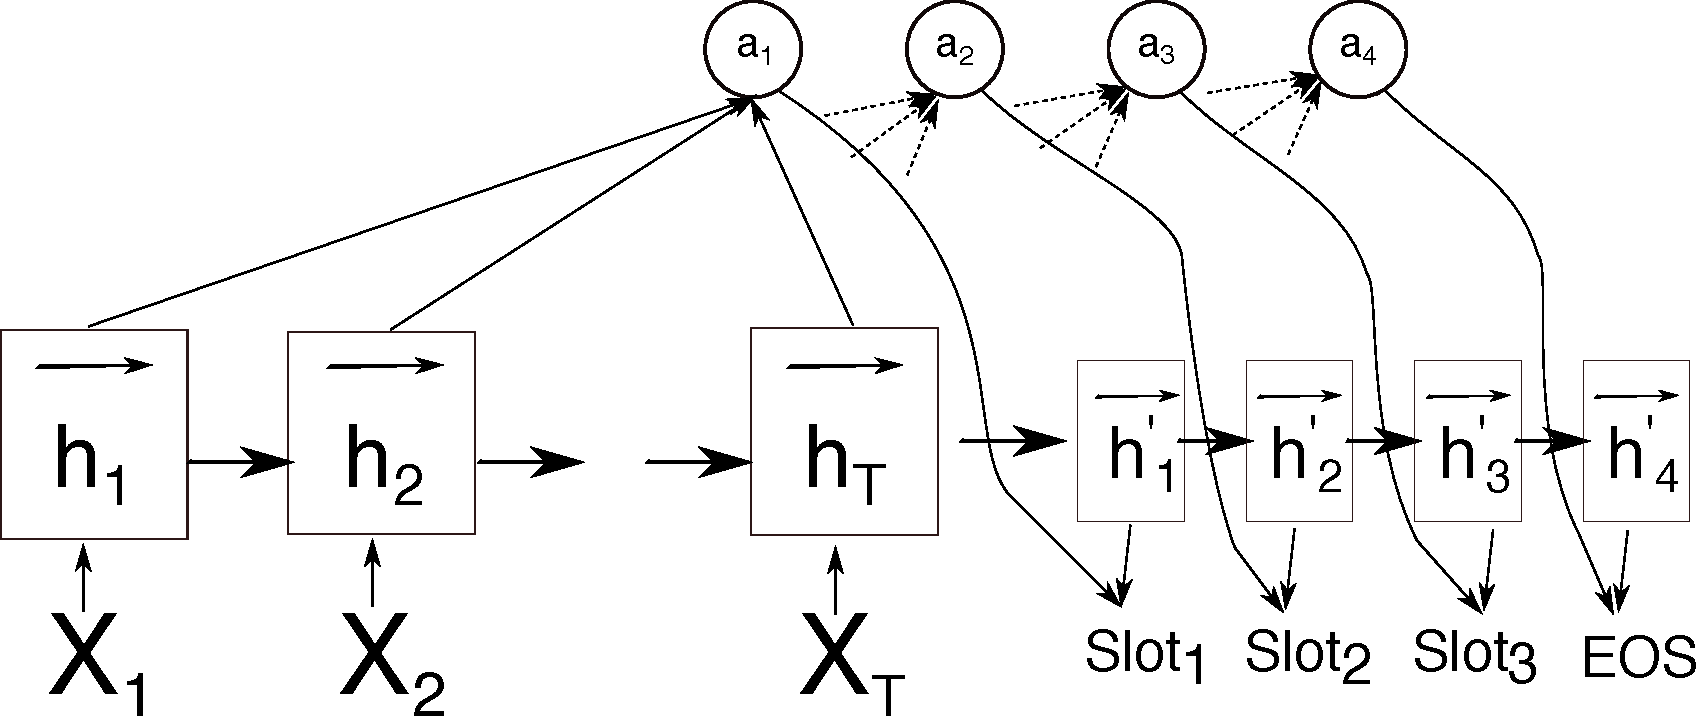
\includegraphics[width=0.7\textwidth]{encdec}
    \end{center}
\end{frame}

\begin{frame}\frametitle{Dialogue state tracking (DST) results}
\begin{center}
% 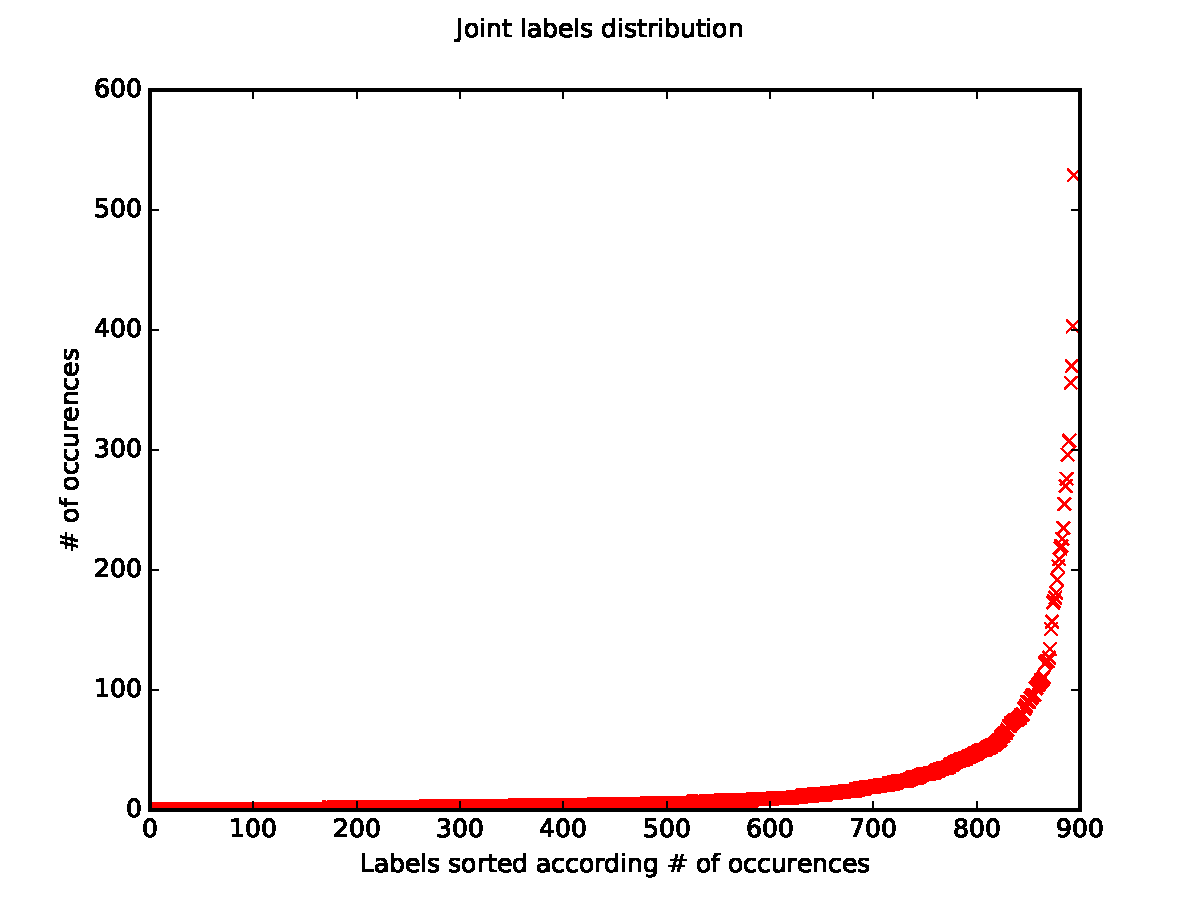
\includegraphics[width=0.6\textwidth]{jointLabelsDistrib} \\
% \includegraphics[width=0.3\textwidth]{DB_features.png} \\
   {\bf No handcrafted ontology needed for abstraction} \\
        Replaced by database features

    {\bf Learned to encode dialogue state into latent space} \\
        Used as a building block for an end-to-end system
    % {\bf Binary features} for each word firing for words are substring of named entity from {\bf database} column. \\
    \vfill
\begin{tabular}{l@{\quad}rll}
\hline
\multicolumn{1}{l}{\rule{0pt}{12pt}
                   {\it Model}}&\multicolumn{1}{l}{\it Dev set}&\multicolumn{2}{l}{\it Test set}\\[2pt]
\hline\rule{0pt}{12pt}
    {\bf \citet{platek2016recurrent} -- EncDec} &   0.867 & 0.730 \\
\hline
    \citet{vodolan_hybrid_2015} & - & 0.745 \\
    \citet{zilka_incremental_2015} & 0.69 & 0.72 \\
    \citet{henderson2013deep} & - & 0.737 \\
\hline
    DSTC2 stacking ensemble~\cite{henderson2014second} & - & 0.789 \\
\hline
\end{tabular}
\end{center}
\end{frame}

\begin{frame}\frametitle{Is explicit dialogue state necessary?}
    \begin{itemize}
        \item For response generation? $\longrightarrow$ {\bf No} {\footnotesize (XY \% OK, 0.XY \% acc)}
        \item For querying database? $\longrightarrow$ {\bf Yes\cite{wen_networkbased_2016} --- Goal eliminate it}
    \end{itemize}
    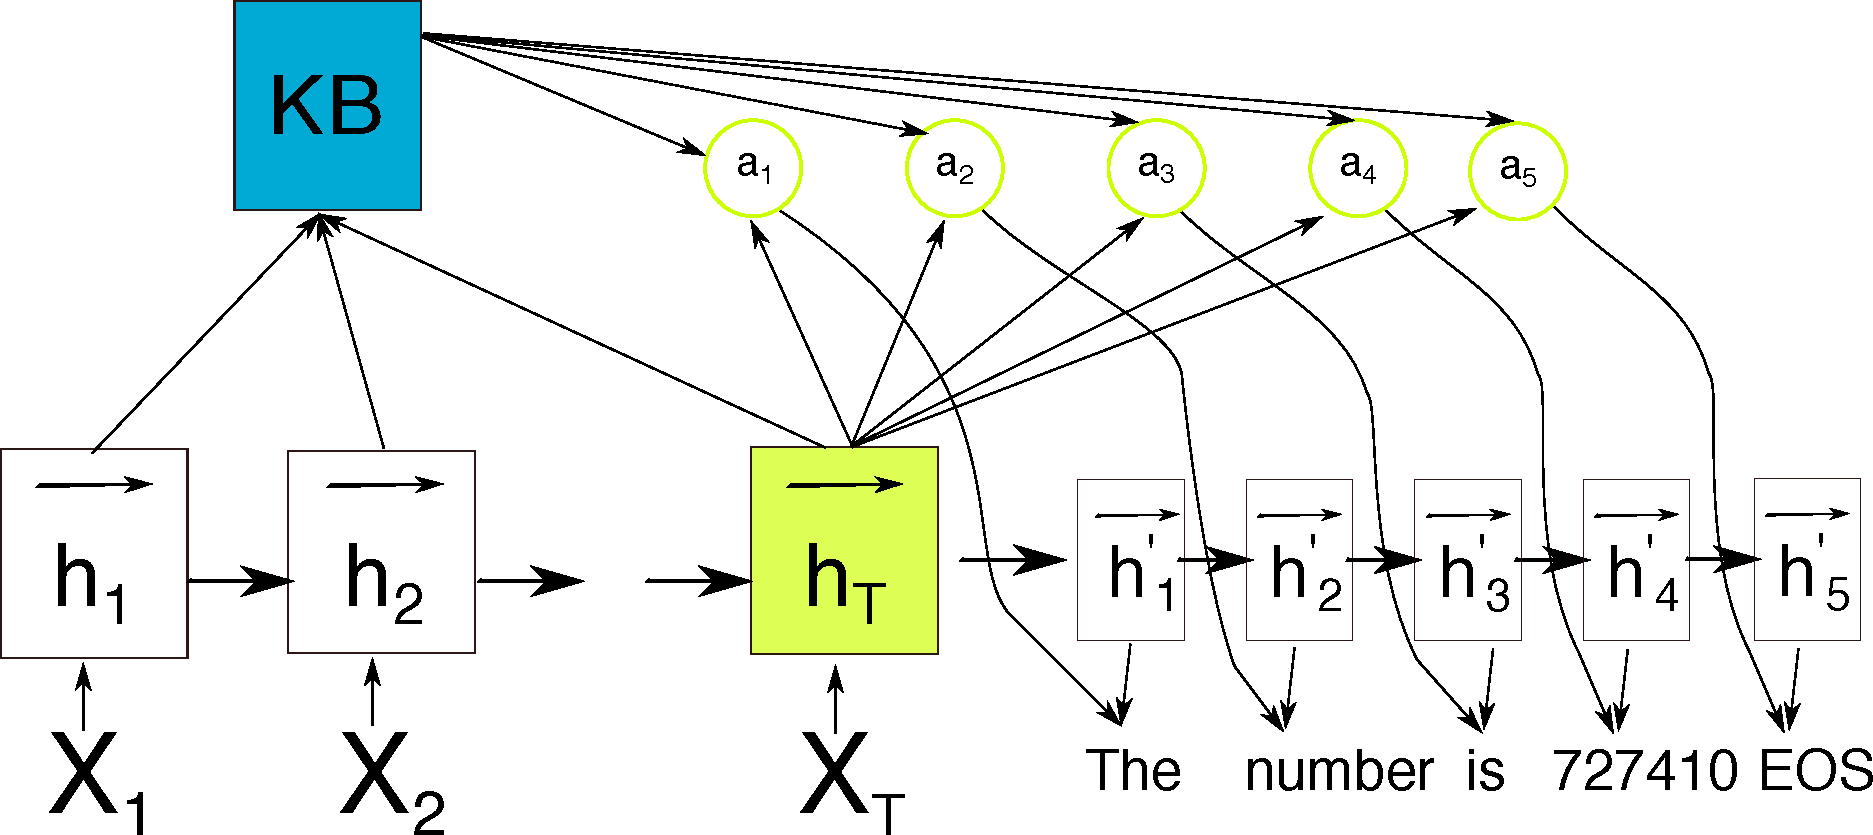
\includegraphics[width=0.7\textwidth]{./encdecdb.pdf} \\
    {\bf input:} {\it anatolia serves turkish food in the moderate price range what is the phone number and address} \\
    {\bf decoded:} {\it The phone number of {\bf meghna} is {\bf 01223 727410} . EOS} \\
    {\bf target:} {\it The phone number of anatolia is {\bf 01223 362372} and it is on 30 Bridge Street City Centre . EOS } \\
\end{frame}

\begin{frame}\frametitle{Human-human conversation collection}
\begin{columns}
\begin{column}{0.45\textwidth}
    {\bf Wizard of Oz} \\
    \begin{itemize}
        \item Communication in real-time 
        \item Hard to pair users and wizards
        \item Wizards respond using a~provided interface
            \begin{itemize}
                \item Wizards training required 
                \item Often still slow  
            \end{itemize}
    \end{itemize}
\end{column}
\begin{column}{0.45\textwidth}
    {\bf Offline collection scheme}
    \begin{itemize}
        \item Workers add one response after reading dialogue history  
        \item Two roles: user and operator 
        \item Annotations mainly from operator
        \item Successfully used for extending DSTC~\cite{wen_networkbased_2016}
    \end{itemize}
\end{column}
\end{columns}
\end{frame}

\begin{frame}\frametitle{Crowd-source worker user interface}
    \begin{center}
    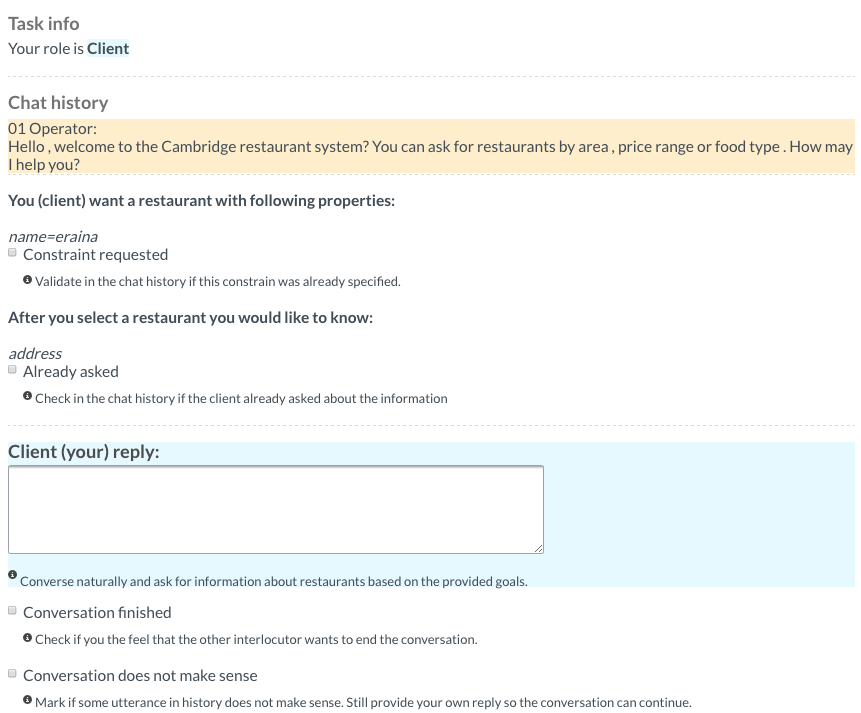
\includegraphics[width=0.85\textwidth]{./gui-annotators-client.png}
    \end{center}
\end{frame}

\begin{frame}\frametitle{Crowd-source worker operator interface}
    \begin{center}
    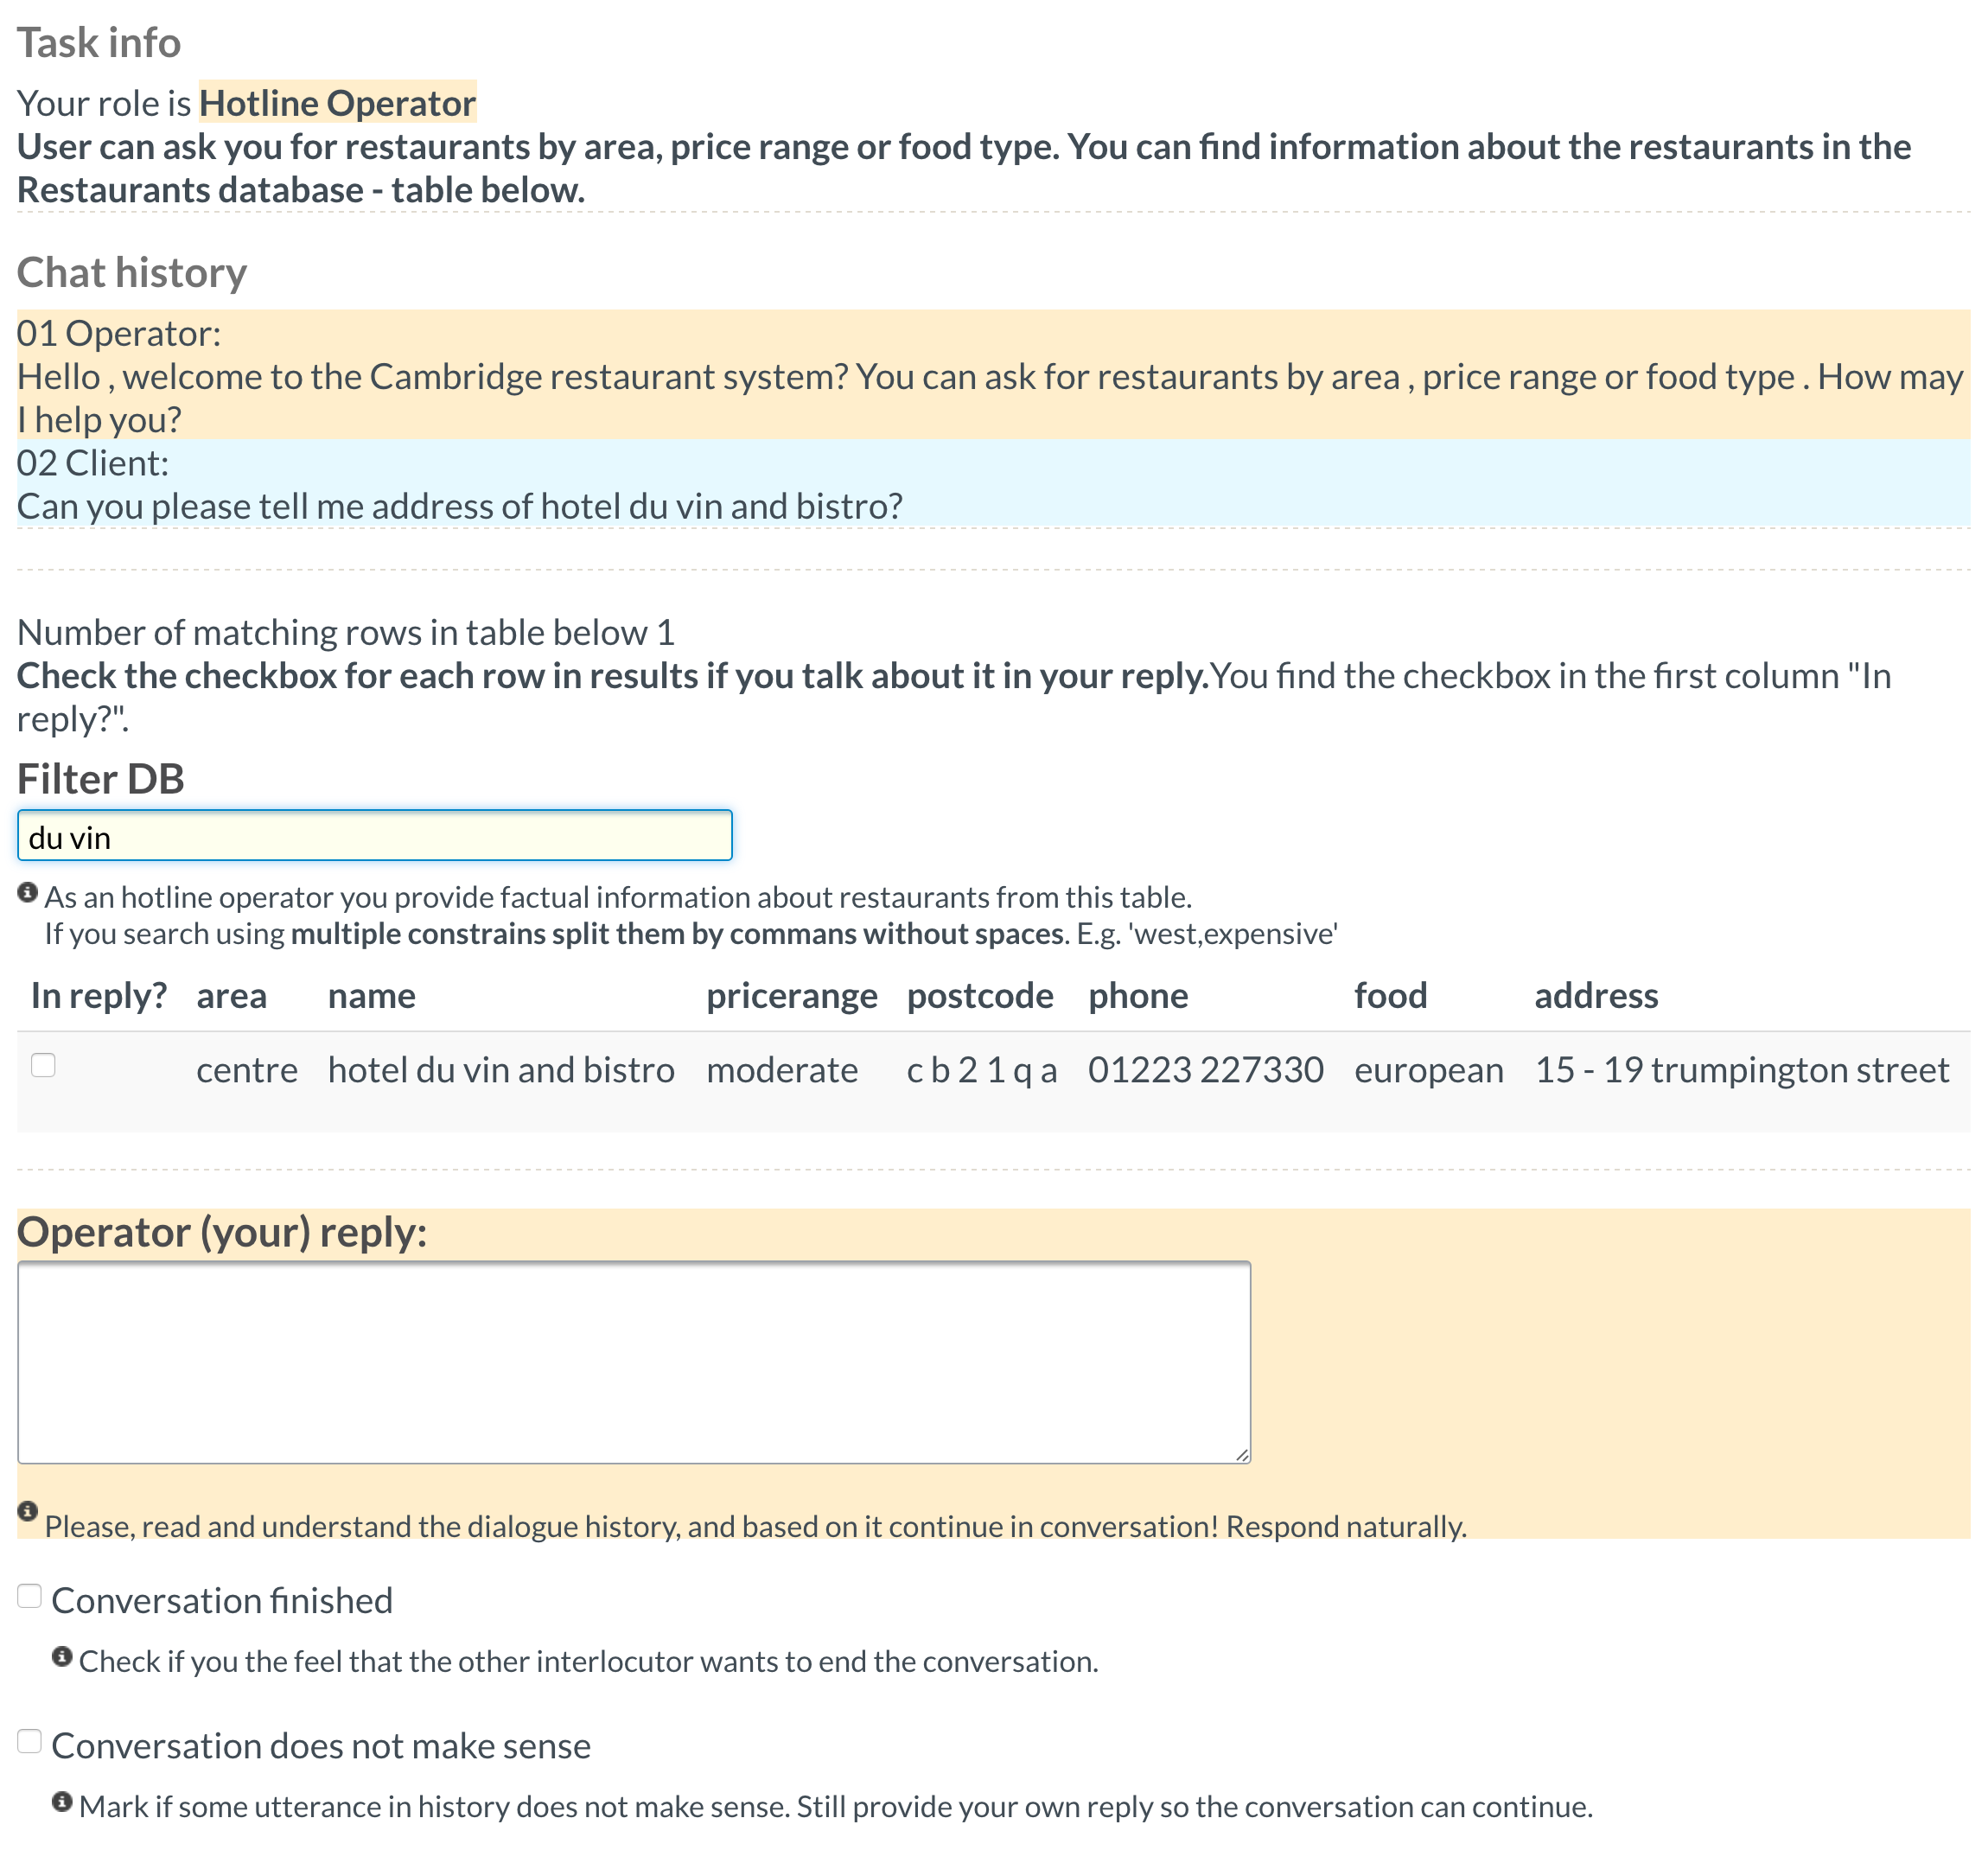
\includegraphics[width=0.85\textwidth]{./gui-annotators-system.png}
    \end{center}
\end{frame}



\section{Research directions}  %%%%%%%%%%%%%%%%%%%%%%%%%%%%%%%%%%%%%%%%%%%%%%%%%%%%%%%%%%%%%%%%

\begin{frame}\frametitle{Data collections in our approach}
    We focus on optimizing neural networks with {\bf minimal annotations}. \ldots A {\bf data hungry} approach. \\
    {\footnotesize \it \dots V textu práce se ale nediskutuje, jestli jsou taková data (v potřebném množství) dostupná, případně jak je získat. Jejich dostupnost je pro další experimentování zásadní.}
    
    {\bf \color{darkgreen} Solution:}\\
    \begin{enumerate}
        \item {\bf Reducing the problem} to a single narrow domain, task oriented (toy) problem.
            \begin{itemize}
                \item \citet{wen_networkbased_2016} showed that 500 dialogues is enough on simplified DSTC2 data
            \end{itemize}
        \item {\bf Crowd-sourcing} -- scalable data collection
        \item Our research topic; How to {\bf bootstrap a system} and start {\bf collecting data and light annotations?}
    \end{enumerate}
\end{frame}


\subsection{End-to-end optimized conversational model}  %%%%%%%%%%%%%%%%%%%%%%%%%%%%%%%%%%%%%%%%%%%%%%%%%%%

\begin{frame}\frametitle{Easy first decoding for dialogue state tracking}
    Using Encoder-decoder RNN with objective for easy-first decoding of~dialogue state labels  \\
    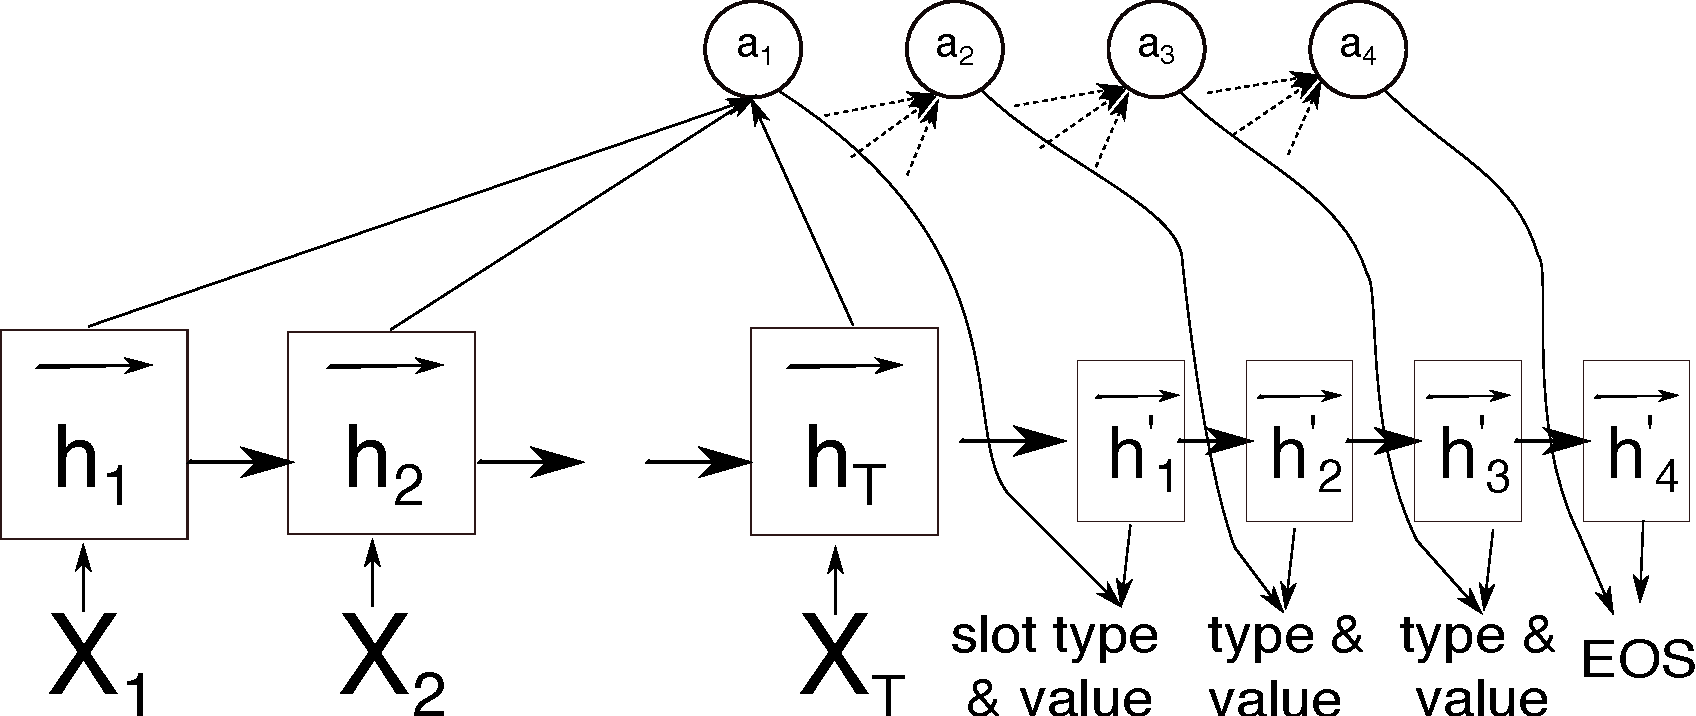
\includegraphics[width=0.6\textwidth]{encdec_easy}
    \begin{itemize}
        \item Experiment to test reinforcement learning algorithms on DSTC2 data
        \item Insight how to combine supervised pre training and reinforcement learning
        \item Further insight into data: What is easy? What is important?
    \end{itemize}
\end{frame}

\begin{frame}\frametitle{Neural network for DB row prediction}
    \begin{center}
    We are able to generate templates \\
    {\bf A correct row required to fill named entities from database}
        \vfill
    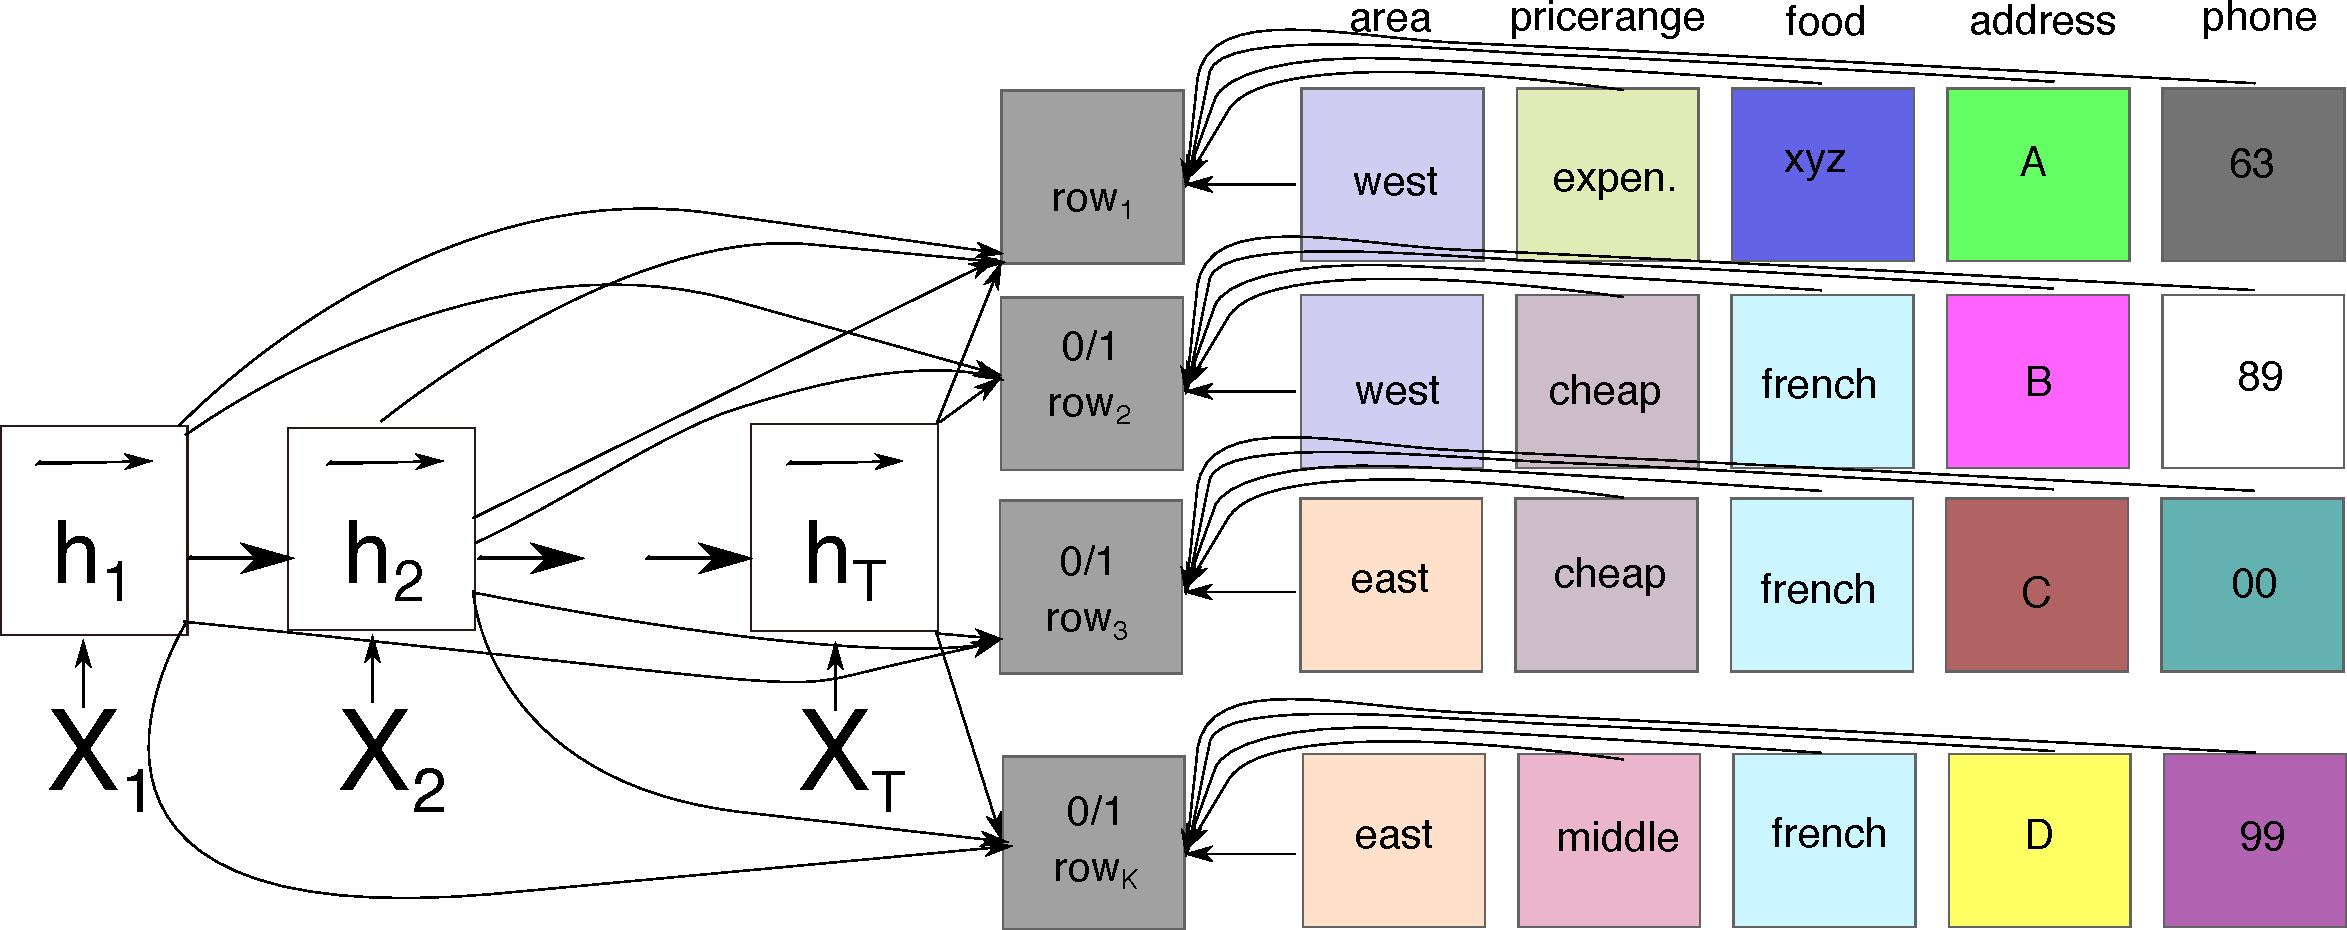
\includegraphics[width=0.85\textwidth]{./e2end_dbclassifiers}
    \end{center}
\end{frame}

\begin{frame}\frametitle{End-to-end NN conversational model}
    {\bf Goal --- Big picture}
    \begin{itemize}
        \item Train joint prediction of response templates and database row prediction 
        \item Fine tune it using Reinforcement Learning (RL) on golden offline data
            \begin{itemize}
                \item Direct evaluation metric optimization
            \end{itemize}
        \item Further obvious experiments
        \begin{itemize}
            \item Access database using standard DB API and train end-to-end model using RL even given non differentiable loss function
            \item Predict reward function/misunderstanding rate using dialogue history and combination of heuristics
            \item Automate annotation collection using active dialogue policy
        \end{itemize}
    \end{itemize}
\end{frame}


\subsection{What next?}  %%%%%%%%%%%%%%%%%%%%%%%%%%%%%%%%%%%%%%%%%%%%%%%%%%%

\begin{frame}\frametitle{Predicting misunderstanding}
    \begin{center}
    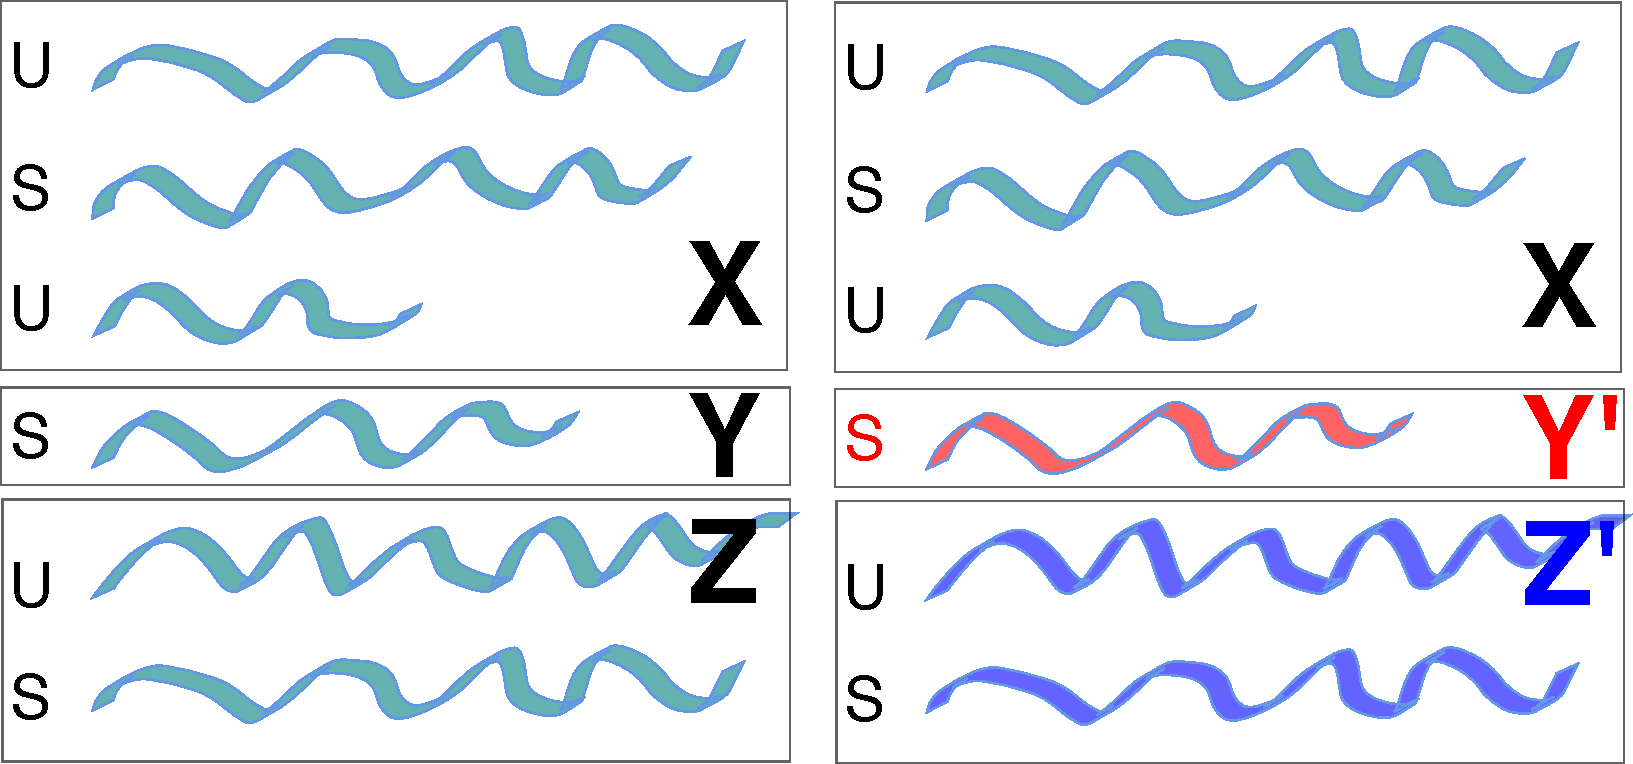
\includegraphics[width=0.7\textwidth]{./misunderstaning}
    \end{center}
    \begin{enumerate}
        \item {\bf Positive examples collection}: Collect followup conversation Z' after artificial nonsensical response Y' \\
        \item {\bf Challenges}: Predict dialogue misunderstanding from single response or very variable follow-up conversation \\ 
        \item {\bf Application}: Handcraft special policies for handling misunderstanding based on the human-human conversations 
    \end{enumerate}
\end{frame}

\begin{frame}\frametitle{Data augmentation through exploration}
    {\bf Problem:}
    \begin{itemize}
        \item Conversations vary a lot after first few turns
        \item Data collection is not targeted to system policy
    \end{itemize}
    {\bf Solution:} \\
    \begin{enumerate}
        \item Use gold data conversations and trained model   
        \item From a conversation select one~system response for a~replacement
            \begin{itemize}
                \item Trained model has to be confident providing alternative
            \end{itemize}
        \item Generate an~alternative response using the model
        \item Collect completely new human-human conversation 
    \end{enumerate}
\end{frame}

\section{Summary}

\begin{frame}\frametitle{Motivation and results}
    \begin{enumerate}
        \item Shift expert work from dialogue policy design to better data collection 
        \begin{itemize}
            \item No handcrafting features for dialogue state tracking~\cite{platek_recurrent_2016}
            \item Feasible (crowd-source) data collection~\cite{platek2016wochat}
        \end{itemize}
        \item Single end-to-end model to optimize
            \item Response generation --- easy (informal experiments)
            \item Database row prediction --- work in progress
            \item Single model -- future work
    \end{enumerate}
\end{frame}

\begin{frame}\frametitle{Future work}
    \begin{enumerate}
        \item Improve problematic (misunderstood) replies
            \begin{itemize}
                \item Detect misunderstanding
                \item Collect more annotation and data examples to handle them better
            \end{itemize}
        \item Improve the end-to-end modeling of dialogue
            \begin{itemize}
                \item Reinforcement learning for optimizing non differentiable evaluation measures directly
                \item Reinforcement learning from delayed and noisy feedback
            \end{itemize}
    \end{enumerate}
\end{frame}



\plain{Thank you for your attention}

\begin{frame}\frametitle{Thank your for your attention}
    {\bf \large \it Questions?} \\
    \vfill
    Content:

  \setbeamertemplate{section in toc}[sections numbered]
  \tableofcontents
    \vfill
    {\footnotesize Slides available at \url{https://github.com/oplatek/extracting-knowledge-from-dialogue-slides}}

\end{frame}

\appendix

\begin{frame}[allowframebreaks]
        \frametitle{References}
        \bibliographystyle{plainnat}
        \bibliography{literature.bib}
\end{frame}

\end{document}
